
\documentclass{article}
\usepackage{graphicx}
%\usepackage{feynmp}
\usepackage{subfigure}
\graphicspath{{figs/}}

\title{Deep Learning Notes}

\author{Peter Thompson}

\begin{document}

\section{random notes}
Don't use sigmoid as an activation function. Tanh is generally superior, as it has a mean of zero (sigmoid has a mean of 0.5). Nonzero mean can make training more difficult in subsequent layers. Tanh has a mean of zero. May want a sigmoid as a final activation function (that is, in the output layer) when doing a binary classification problem.

relu is generally good.



\section{notation}
\section{logstic loss}

loss function is the loss/error associated with a single training example
Cost function is the loss computed over all examples

logistic loss

Think of $\hat{y}$ as the conditional probability $\hat{y}(x) = P(y=1|x)$. The probability $y=0$ is then $P(y=0|x) = 1 - \hat{y}$. These two outcomes can be summarised as
\begin{equation}
P(y|x) = \hat{y}^y(1-\hat{y})^{(1-y)}
\end{equation}
The above is for a single example. The likelihood (of parameters) for a given training set would be obtained from the product $\prod_i P(y_i|x_i)$, where $\hat(y)_i$ is a function of $x_i$.

The expression for logistic loss can then be obtained from the negative log likelihood of $P(y|x)$ above
\begin{equation}
L = \sum_i  (y_i-1) ln(1 - \hat{y}_i) - y_i ln(\hat{y}_i)
\end{equation}
The log of the product reduces to a sum over logs.



\section{activation functions and their derivatives}


\subsection{sigmoid}
Sigmoid used to be the default activation function, but in recent times ReLu has proven to be more popular/perform better. Sigmoid is still good for an output function (i.e. activation function in the output layer) in binary classification tasks.
The sigmoid function (or logit function) and its derivative are given by
\begin{eqnarray*}
\sigma(x) & = &\frac{1}{1 - e^{-x}} \\
\frac{d\sigma(x)}{dx} & = & \sigma(x)(1 - \sigma(x)) \\
\end{eqnarray*}

these are plotted below
\begin{figure}[tb]
\begin{centering}
\subfigure{
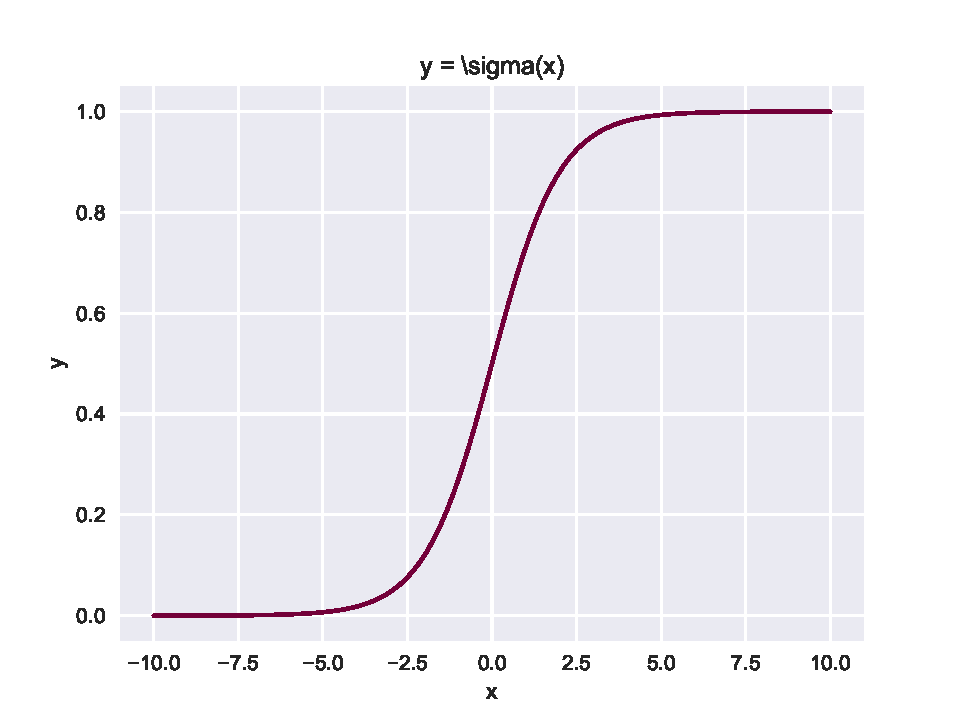
\includegraphics[width=0.45\linewidth,angle=0]{sigmoid.pdf}
% \caption{sigmoid activation function}
}
\subfigure{
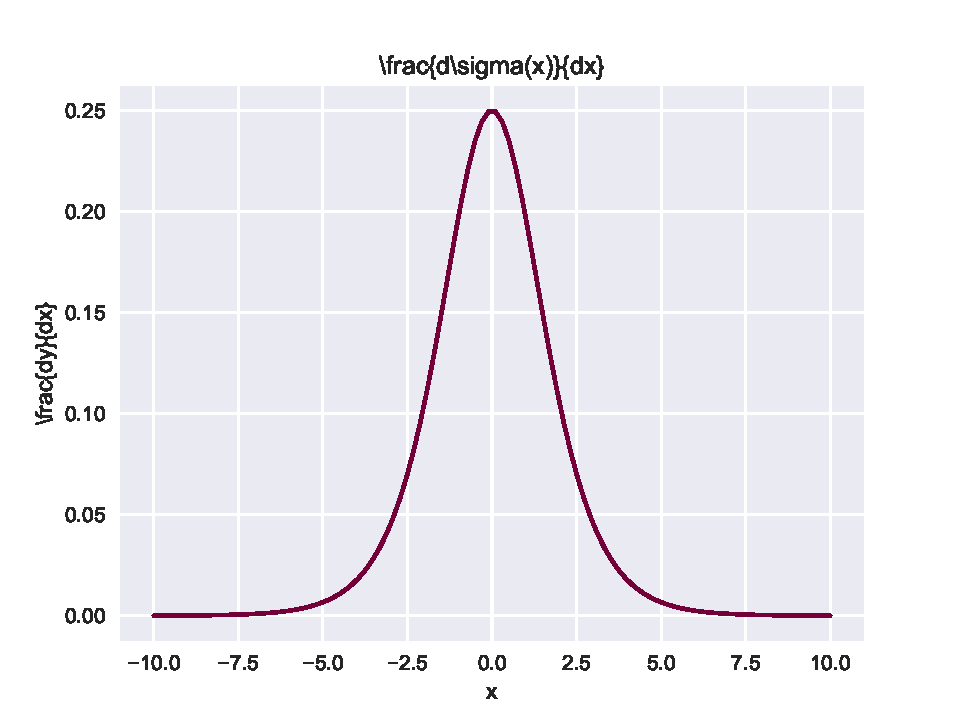
\includegraphics[width=0.45\linewidth,angle=0]{sigmoid_derivative.pdf}
% \caption{sigmoid derivative}
}
\end{centering}
\end{figure}

\subsection{tanh}
Tanh is good. It's a nonlinear function, like sigmoid, but for zero input it returns zero output. The mean of this function (given uniform x) is zero, so it handles centred data very well ( zero input gives zero output).
The tanh function (sinh/cosh) and its derivative are given by
\begin{eqnarray*}
\mathrm{tanh}(x) & = &\frac{e^x\,-\, e^{-x}}{e^x\,+\, e^{-x}} \\
\frac{d\sigma(x)}{dx} & = & 1 - \mathrm{tanh}^2(x) 
\end{eqnarray*}

these are plotted below
\begin{figure}[tb]
\begin{centering}
\subfigure{
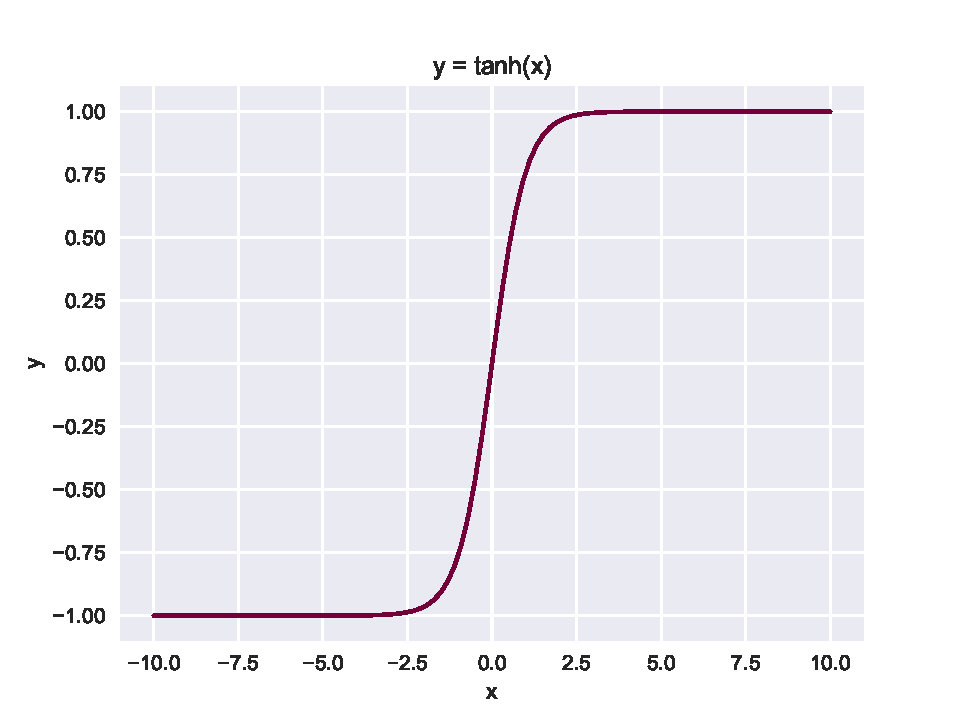
\includegraphics[width=0.45\linewidth,angle=0]{tanh.pdf}
% \caption{tanh activation function}
}
\subfigure{
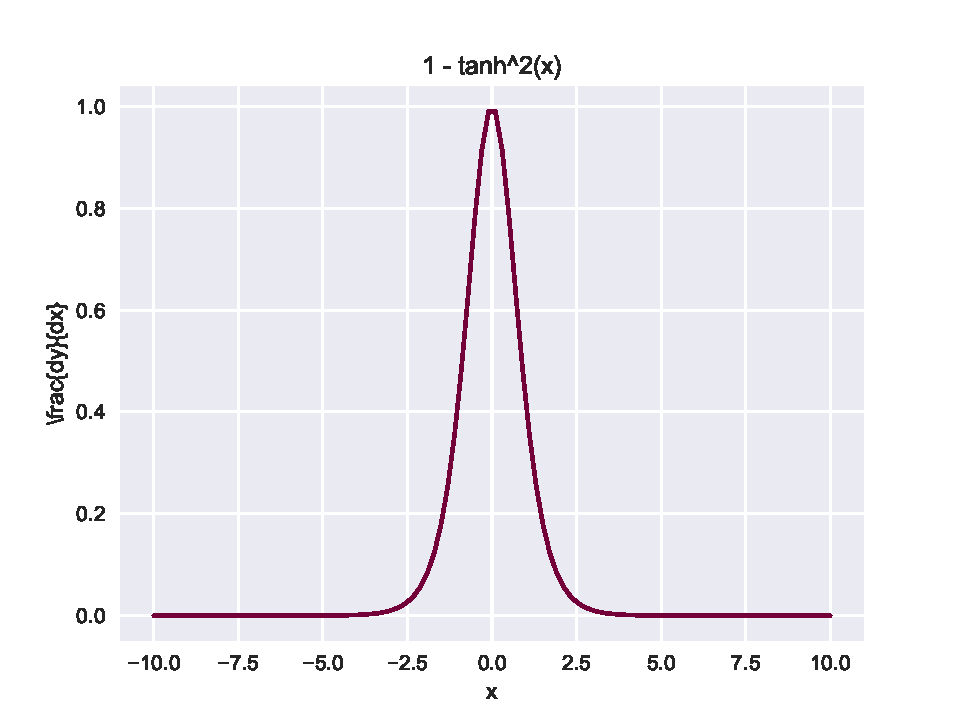
\includegraphics[width=0.45\linewidth,angle=0]{tanh_derivative.pdf}
% \caption{tanh derivative}
}
\end{centering}
\end{figure}

\subsection{ReLu}
rectified linear unit. Max(0,x). This is a very popular activation, as it tends to give good results. Should in general be the first choice for an activation function (rather than sigmoid/tanh, though there may be cases where these perform better).
\begin{figure}[tb]
\begin{centering}
\subfigure{
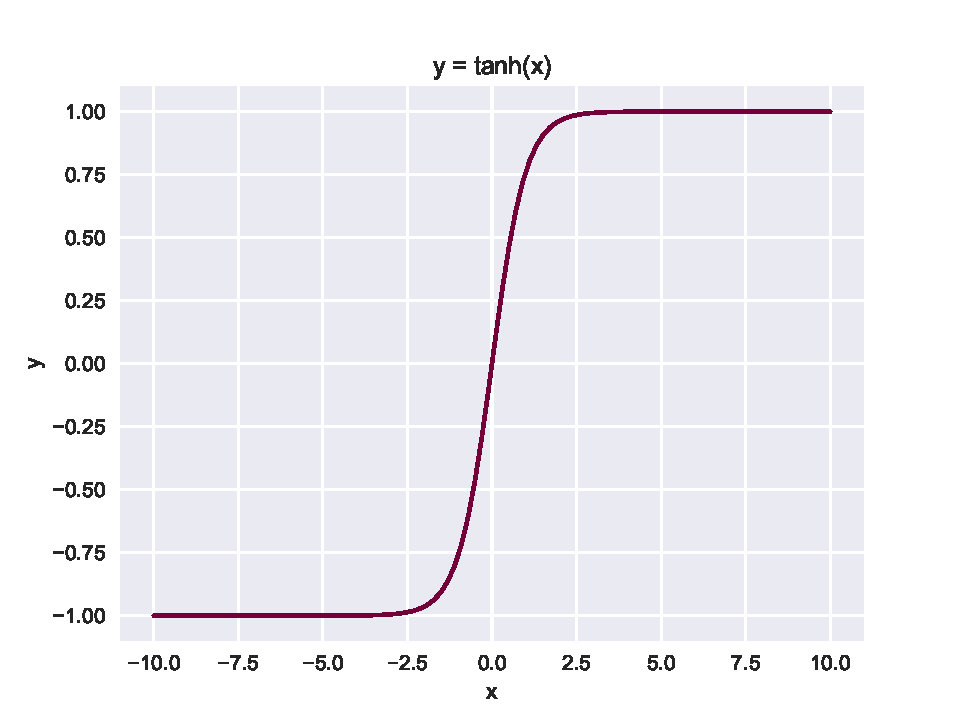
\includegraphics[width=0.45\linewidth,angle=0]{tanh.pdf}
% \caption{tanh activation function}
}
\subfigure{
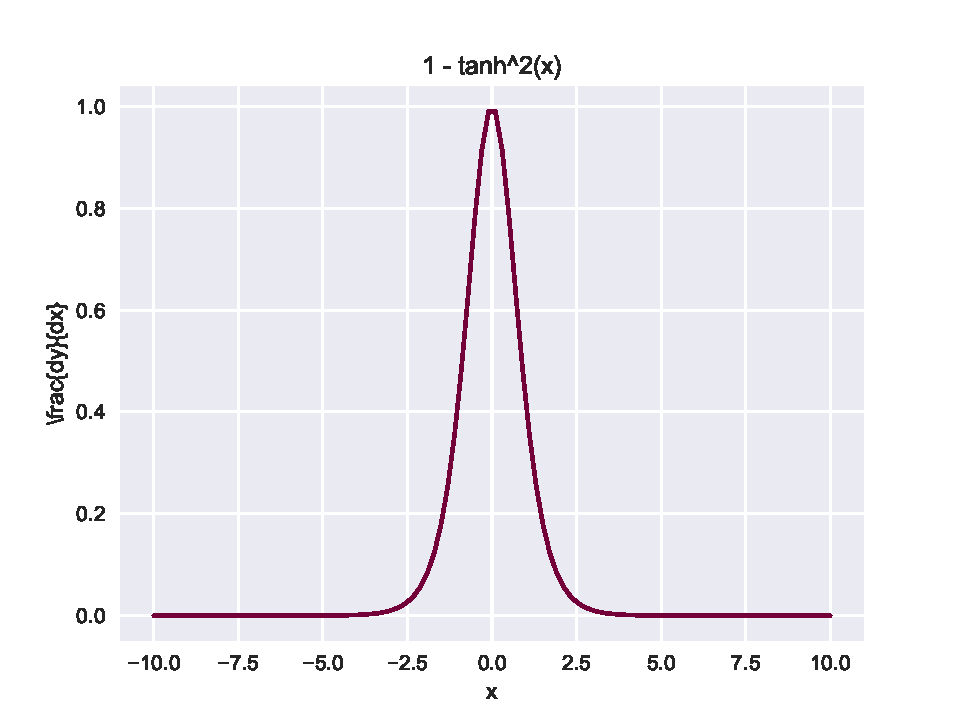
\includegraphics[width=0.45\linewidth,angle=0]{tanh_derivative.pdf}
% \caption{tanh derivative}
}
\end{centering}
\end{figure}

\subsection{leaky ReLu}
Gradient saturation and such. If a Relu Network ever gets to a state where the inputs are large and negative, all the gradients will vanish, and the network will stop updating, it gets stuck. Leaky Relu has a very small (1\%) output for negative x, so the gradient never fully vanishes. It's a little more robust
\begin{figure}[tb]
\begin{centering}
\subfigure{
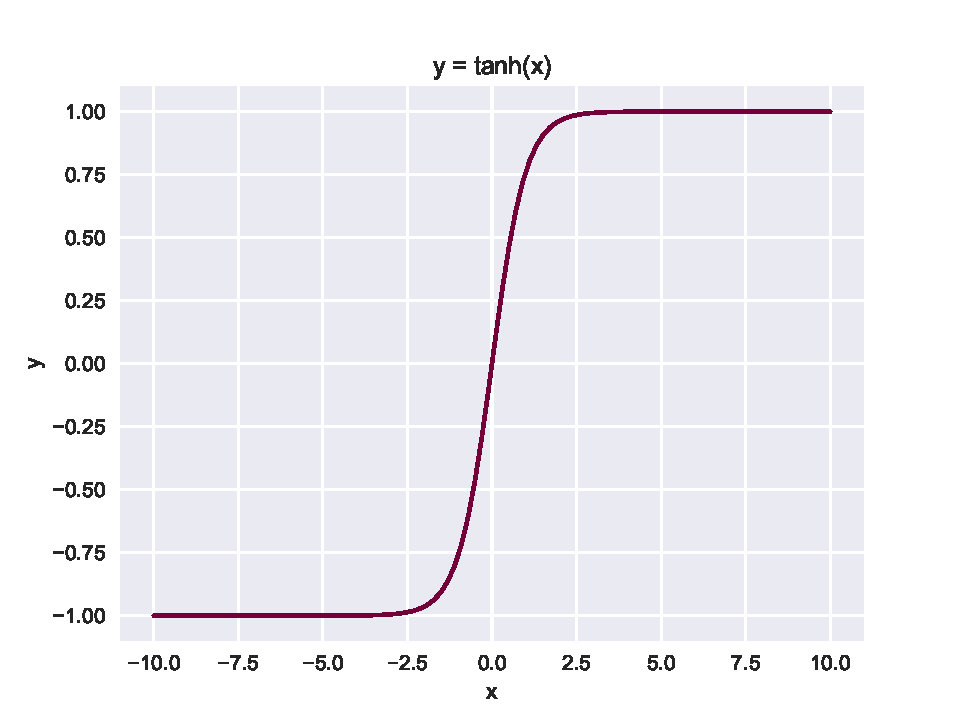
\includegraphics[width=0.45\linewidth,angle=0]{tanh.pdf}
% \caption{tanh activation function}
}
\subfigure{
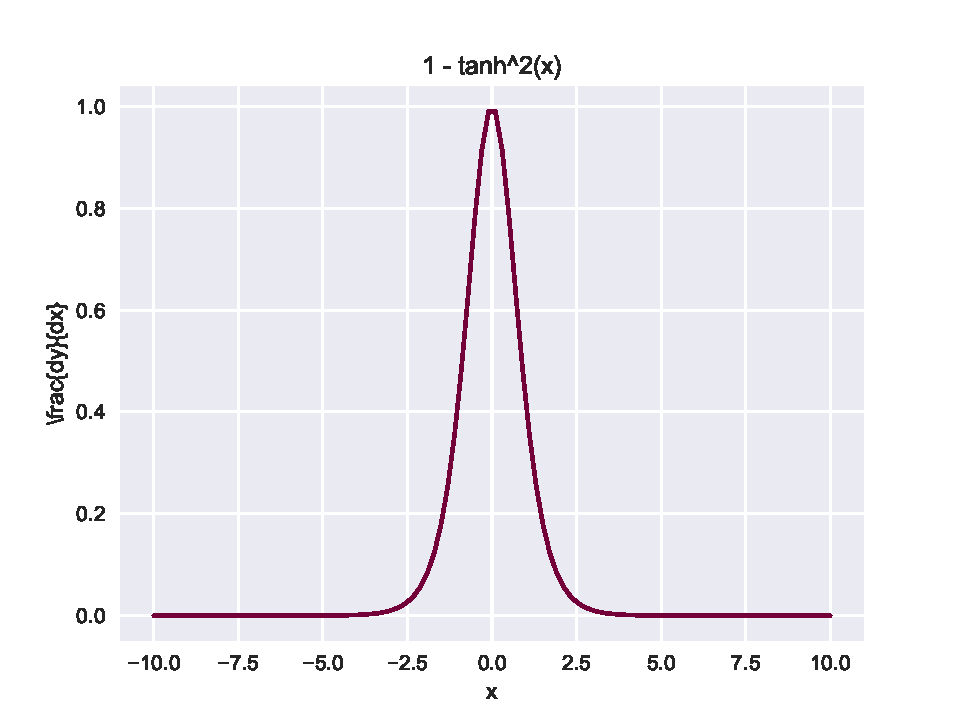
\includegraphics[width=0.45\linewidth,angle=0]{tanh_derivative.pdf}
% \caption{tanh derivative}
}
\end{centering}
\end{figure}
\end{document}

